\documentclass[a4paper]{article}
\usepackage{xeCJK}
\usepackage{hyperref}
\usepackage{indentfirst}
\usepackage{listings}
\usepackage{graphicx}
\usepackage{amsmath}
\setlength{\parindent}{2em}
\title{基于支持向量机的汽油辛烷值定量分析}
\author{FukoMaster}
\begin{document}
	\maketitle
	
	\begin{abstract}
		content...
	\end{abstract}
	
	\tableofcontents
	
	\section{引言}
		汽油辛烷值是衡量汽油在气缸内抗爆震燃烧能力的一种指标,其值的高低意味着抗爆性的好坏。汽油在气缸中爆震燃烧时引起气缸温度剧升、汽油燃烧不完全、机器强烈震动,从而使输出功率下降,并容易造成机件受损。
		
		目前快速检测汽油辛烷值的方法主要有有红外光谱法、气相色谱法等。近红外光谱法由于成本低廉、速度快、无排放物等优点,逐渐成为车用汽油辛烷值测定的主流技术。然而由于近红外光谱的测量结果维数较多,各维度间具有一定程度的相关性,因此数据的分析处理则较为困难,基本的统计学方法如线性回归、主成分分析等效果一般。
		
		支持向量机 (Support Vector Machine, SVM) 是 Corinna Cortes 和 Vapnik 等于 1995 年首先提出的,它在解决小样本、非线性及高维模式识别中表现出许多特有的优势,并能够推广应用到函数拟合等其他机器学习问题中。支持向量机能够根据有限的样本信息在模型的复杂性和学习能力之间寻求最佳折中,以求获得较好的适应能力。
		
	\section{工作环境}
		本文使用的软件平台如下:
		
		\begin{itemize}
			\item openSUSE Tumbleweed + Linux Kernel 4.13.9
			\item Python 3.6 + pip
			\item libsvm
			\item Keras + TensorFlow
		\end{itemize}
	
		\subsection{openSUSE Tumbleweed + Linux Kernel 4.13.9}
			Linux 是一套开源的类 Unix 操作系统,它遵循 POSIX 标准,并具有对多用户、多任务、多线程和多CPU的支持。 
			openSUSE 则是基于 Linux 的发行版中的一套,其界面较为友好,比较易于使用。
		\subsection{Python}
			Python 是一种面向对象的解释型计算机程序设计语言,其源代码和解释器 CPython 遵循 GPL (GNU General Public License) 协议开源。
			Python 对科学计算具有良好的支持,拥有诸如 NumPy 、 SciPy 、 MatPlotLib 等诸多开源代码库。
			另外,它还能轻松的调用来自其他语言(比如C)所编写的库,即便于代码复用,还可以提高关键代码的运行速度。
		\subsection{libsvm}
			libsvm是台湾大学林智仁 (Lin Chih-Jen) 教授等开发设计的一个简单、易于使用和快速有效的SVM模式识别与回归的软件包,提供了包括C/Java/Python/MATLAB等大量接口,并基于 BSD 协议开源,其代码托管于\url{https://github.com/cjlin1/libsvm}。
			由于作者未通过PyPI提供包,需要参照手册自行编译并安装。
		\subsection{Keras + TensorFlow}
			TensorFlow 最初由 Google 大脑小组的研究员和工程师们开发出来,用于机器学习和深度神经网络方面的研究,但这个系统的通用性使其也可广泛用于其他计算领域。它灵活的架构让你可以在多种平台上展开计算,例如台式计算机中的一个或多个CPU(或GPU),服务器,移动设备等等。
			
			Keras 是一个高层神经网络 API , Keras 由纯 Python 编写而成并基于 Tensorflow 、 Theano 以及 CNTK 后端。Keras 为支持快速实验而生,能够把你的idea迅速转换为结果,具有高度模块化,极简,和可扩充特性,非常适合于简易和快速的原型设计。
			
	\section{数据预处理}
		光谱仪所采集的原始光谱图,除了受样品自身的基团组成与含量影响外,还会被样品颜色与杂质、检测器噪声所干扰。此外,光源强度、探头与样品的矩离、检测器灵敏度等因素也影响着光谱的强度。因此在对光谱进行建模前,需要通过适当的手段进行预处理,以便消除光谱数据中与样品基团组成无关的信息。
		
		本文使用的汽油 NIR 光谱数据如图\ref{fig:nir-data-raw}所示。
		
		\begin{figure}[h]
			\centering
			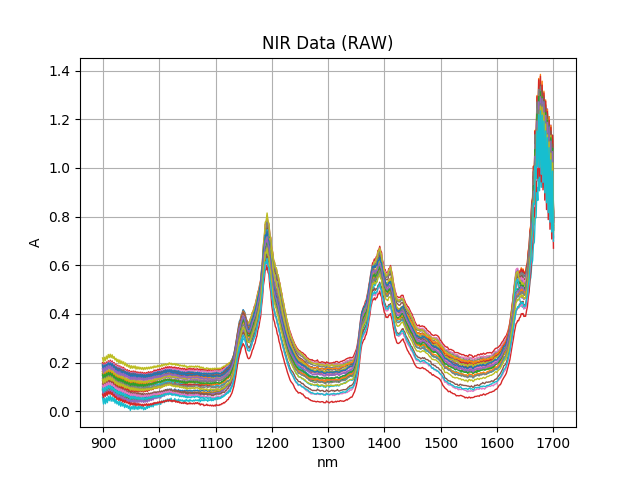
\includegraphics[width=\linewidth]{../img/raw}
			\caption{原始光谱数据}
			\label{fig:nir-data-raw}
		\end{figure}
	
		\subsection{平滑}\label{section:filter}
			与图像处理或时域信号的预处理方式不同,光谱一般采用多项式卷积平滑进行预处理。
			多项式卷积平滑是通过对移动窗口内的数据进行多项式最小二乘拟合,以拟合值代替原始数据点,减少原始数据所含噪声对谱图的影响,达到平滑之目的。
			
			假设移动窗口的中心波长为 k ,半宽为 h ,再假定使用二次多项式进行拟合,则可以按公式 \eqref{equ:filter}来计算拟合参数。
			
			\begin{equation}\label{equ:filter}
				\beta_{LS}(k) = 
				\begin{bmatrix}
					a_0(k) \\ a_1(k) \\ a_2(k)
				\end{bmatrix}
				= \left( A(h)^TA(h) \right)^{-1}A(h)^TX(k) = 
				\begin{bmatrix}
					f_0(h) \\ f_1(h) \\ f_2(h)
				\end{bmatrix} 
				X(K)
			\end{equation}
			其中:
			\[
				A(h) =
				\begin{bmatrix}
					1 & -h & h^2 \\
					\vdots & \vdots & \vdots \\
					1 & 0 & 0 \\
					\vdots & \vdots & \vdots \\
					1 & h & h^2 \\
				\end{bmatrix} 
			\]
			
			在计算出拟合参数后,该点在平滑后的值则由公式\eqref{equ:filter2}得出。
			对图\ref{fig:nir-data-raw}中的数据进行平滑,取移动窗口半宽 $h = 5nm$ 得到的结果如图\ref{fig:filter}所示。
			可以看到,相比于图\ref{fig:nir-data-raw}中的原始数据,多项式卷积平滑有效的降低了噪声。
			
			\begin{equation}\label{equ:filter2}
				x_f(k) = a_0(k) = f_0(h)X(k)
			\end{equation}
			
			\begin{figure}[h]
				\centering
				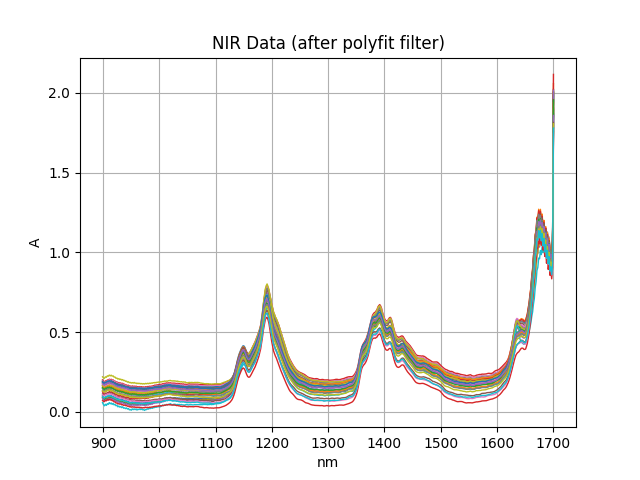
\includegraphics[width=\linewidth]{../img/filter}
				\caption{光谱数据多项式卷积平滑结果}
				\label{fig:filter}
			\end{figure}
			
		\subsection{基线校正}
			由于光谱法一次测量的时间相对较长,若在这段时间内,各器件的特性可能会逐渐发生微小变化,这就会造成基线漂移。
			
			出于模型的健壮性考量,假定基线只发生了线性漂移,因此这里多次使用了一次多项式拟合进行迭代。对于每次拟合,可以认为原始数据落在拟合直线上方,且偏差超过拟合结果的均方根误差 (RMSE) 的点一定不属于基线,因此需要在下次拟合时忽略这些点;而其他的点则可能属于基线,应当参与下次拟合。随着迭代的进行,剔除的不属于基线的点越来越多,拟合结果也越来越靠近真实的基线。当拟合的均方根误差 (RMSE) 接近仪器的准确度时,继续迭代则会剔除掉原本属于基线的点,造成基线的偏离,因此应当停止迭代。
			
			基线校正的结果如图\ref{fig:baseline}所示,与图\ref{fig:nir-data-raw}所示的原始数据相比,各牌号汽油的光谱曲线均大致重合,较为符合实际情况。
			
			\begin{figure}[h]
				\centering
				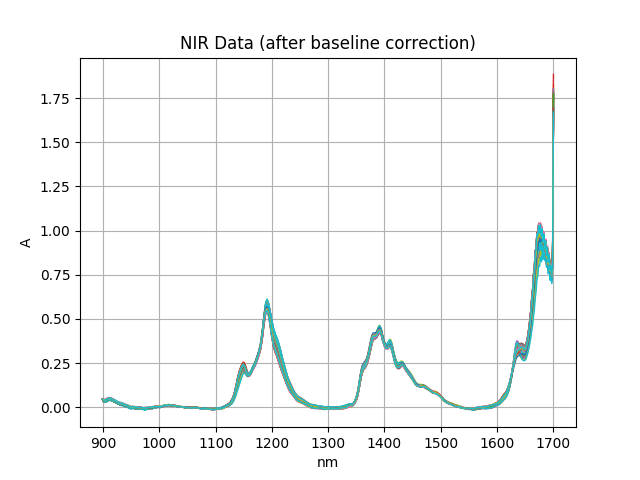
\includegraphics[width=\linewidth]{../img/baseline}
				\caption{光谱数据基线校正结果}
				\label{fig:baseline}
			\end{figure}
			
		\subsection{微分}
			由于光谱数据的噪声较大,不太适合直接进行微分运算,因此需要先进行多项式平滑,然后再微分。多项式平滑的方法在第\ref{section:filter}节中已有叙述,只需在使用公式\ref{equ:filter2}计算输出值前,对拟合函数进行微分即可。
			
			因此首先使用公式\ref{equ:filter}计算每个中心波长的拟合参数,然后用公式\eqref{equ:diff}计算光谱当前波长的一阶微分值,或用公式\eqref{equ:diffdiff}计算光谱当前波长的二阶微分值。
			
			\begin{equation}\label{equ:diff}
				\frac{d\hat{x}(k+t)}{dt}\bigg|_{t=0}
				= a_1(k) =
				f_1(h)X(k)
			\end{equation}
			
			\begin{equation}\label{equ:diffdiff}
				\frac{d^2}{dt^2}\hat{x}(k+t)
				= 2a_2(k) =
				2f_2(h)X(k)
			\end{equation}
			
			光谱一阶微分后的结果如图\ref{fig:diff}所示,由于一阶微分获取的是变化量,因此除了滤波外,还消除了基线漂移的影响。
			
			\begin{figure}
				\centering
				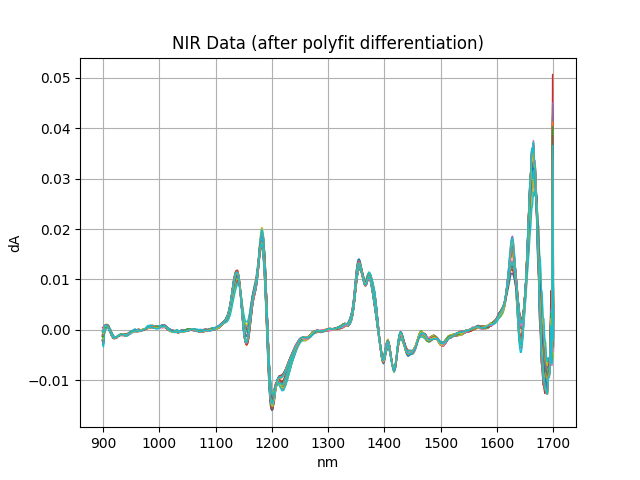
\includegraphics[width=\linewidth]{../img/diff}
				\caption{光谱数据一阶微分结果}
				\label{fig:diff}
			\end{figure}
			
		\subsection{相关性分析}
			相关性分析用于考察光谱信息与待测参数的相关程度。若光谱各频率与待测参数的相关性均非常低,那么无论使用什么算法,通过分析光谱数据来获得待测参数都会非常困难。
			
			取每一个波长的数据,根据公式\eqref{equ:correlation}计算该波长上数据的相关性,其结果如图\ref{fig:correlation}所示。可以看到,在许多波长上,吸光度的一阶微分与待测参数的相关性显著,甚至在 1220nm 附近达到了 1 ,因此可以认为通过光谱来测量待测参数是可行的。
			
			\begin{equation}\label{equ:correlation}
				\rho_{XY} = \frac{Cov(X, Y)}{\sqrt{D(X)D(Y)}}
			\end{equation}
			\begin{figure}
				\centering
				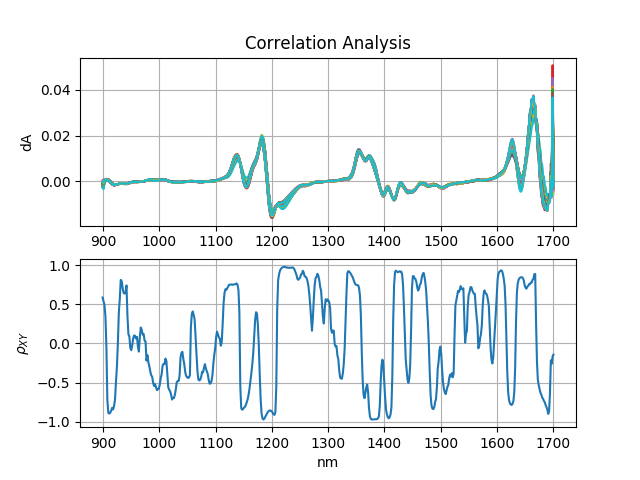
\includegraphics[width=\linewidth]{../img/correlation}
				\caption{一阶微分的相关性分析}
				\label{fig:correlation}
			\end{figure}
			
	\section{支持向量回归}
		支持向量机是用来解决二分类问题的一种模型,其基本思想是利用核函数,将线性不可分的数据集映射到高维空间,然后在高维空间中寻找一个超平面,使得数据集线性可分。
		
		
	\section{卷积神经网络}
	\section{总结}
\end{document}